
\section{Supporting Flyspeck in a Semantic Wiki}

Our focus in this work is on making the extent and structure of Flyspeck
comprehensible, communicating where work needs to be done, and allowing
collaborators to improve the structure and finally to contribute computerized
proofs.  \claim{For this the outline of the whole proof from the
book~\cite{Hales:2008:FlyspeckBook} needs to be represented in the wiki, where
the mathematical statements (including definitions, lemmas, and theorems) are
available in a human-readable way (with formulae in \LaTeX\ or presentational
MathML) as well as a computerized presentation suitable for using in a theorem
prover.}  In order to obtain a well-structured network of knowledge items, each
mathematical statement should be presented on one wiki page, which shows its
human-readable representation taken from the book, offers additional space for
annotation, and allows for downloading a formal representation.  Here, we are
not yet considering formal proof checking \emph{inside} the wiki, but rather
using the wiki for communication about the projects and annotation of informal
text.

% \subsection{Motivation}
% \label{sec:req}

% The Flyspeck project has garnered significant enthusiasm in the theorem proving
% community: Hales has given talks about the project at a number of prestigious
% conferences, and aspects of Flyspeck are currently a motivation behind 
% one complete and at least
% two current PhD dissertations.  At present, however, Flyspeck is not ready for
% crowdsourcing.  

\subsection{Scenario}

\begin{scenario}
An example usage scenario is as follows (cf.\ fig.~\ref{fig:pagestructure}). A
user wishes to contribute to Flyspeck.  She looks at our wiki main page, which
shows her what still needs to be done.  Preferring trigonometry, she searches
for open problems in that field.  This returns a list of lemmas related to
analysis from which she can choose one that seems possible given her time
constraints. She reads the text of a paper proof culled from Hales' book and
annotated by other wiki collaborators and downloads the relevant formal
definitions and lemmas.  She uses a proof assistant to begin formalizing the
paper proof.  At some point, she needs clarification on some definition and
additionally has an idea on how to generalize this lemma.  She thus asks for
help, makes comments on the discussion pages of the wiki, and refines the
annotations of the lemma.  She completes her proof, and uploads the proof
assistant file to the wiki.  The wiki uses a theorem prover to check the proof
for correctness and, if it is correct, adds it to the database.

\newcommand{\wikipage}[6]{\node[draw,text width=4cm,font=\tiny\sffamily,#6] (#1) at #2 {
    {\scriptsize\bfseries #3}\\
    #4
    ~\\[1em]
    [Download Twelf representation]\\
    #5
  };}
\newcommand{\dummywikipage}[2]{\wikipage{#1}{#2}{\textcolor{red!20}{Cosine}}{\textcolor{red!20}{$\cos$}}{
      \textcolor{red!20}{Page type: Definition\\
      Topic: Trigonometry}
    }{fill=red!20}}
\begin{figure}
  \centering
  %\vspace{-.5cm}
  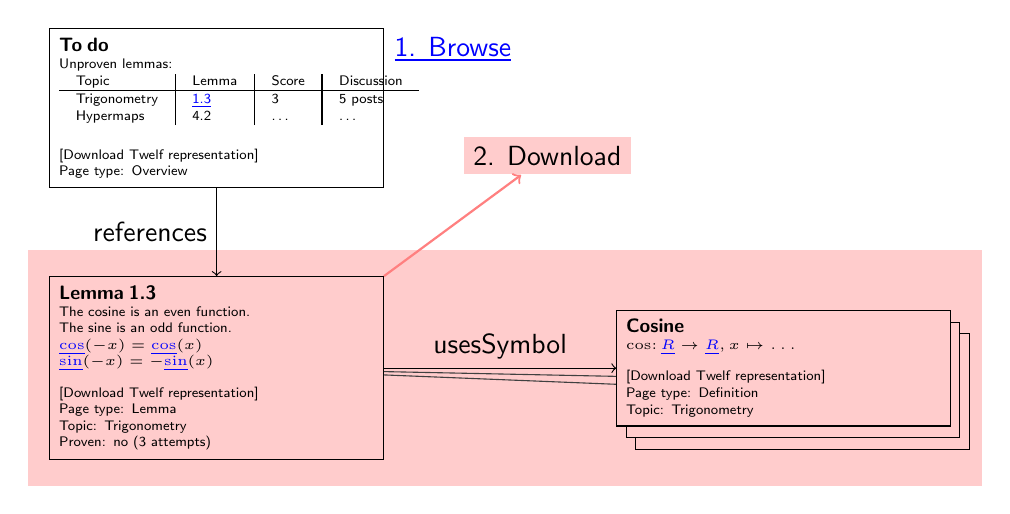
\begin{tikzpicture}[set style={{default}+=[scale=1.5,font=\sffamily]},default,xscale=.8]
    \fill[red!20] (-2.0,-1.0) rectangle (8.1,1.0);
    \wikipage{lemma}{(0,0)}{Lemma 1.3}{The cosine is an even function.\\
      The sine is an odd function.\\
      ${\color{blue}\underline{\cos}}(-x)={\color{blue}\underline{\cos}}(x)$\\
      ${\color{blue}\underline{\sin}}(-x)=-{\color{blue}\underline{\sin}}(x)$}{Page type: Lemma\\
      Topic: Trigonometry\\
      Proven: no (3 attempts)}{fill=red!20}
    \dummywikipage{tan}{(6.2,-0.2)}
    \draw[black!75] (lemma) -- (tan);
    \dummywikipage{sin}{(6.1,-0.1)}
    \draw[black!75] (lemma) -- (sin);
    \wikipage{cos}{(6,0)}{Cosine}{$\cos\colon{\color{blue}\underline{\mathbb{R}}}\to{\color{blue}{\underline{\mathbb{R}}}},x\mapsto\ldots$}{
      Page type: Definition\\
      Topic: Trigonometry
    }{fill=red!20}
    \wikipage{todo}{(0,2.2)}{To do}{Unproven lemmas:
      \begin{tabular}{l|l|l|l}
        Topic & Lemma & Score & Discussion \\
        \hline
        Trigonometry & \textcolor{blue}{\underline{1.3}} & 3 & 5 posts \\
        Hypermaps & 4.2 & \ldots & \ldots 
      \end{tabular}
    }{
      Page type: Overview
    }{}
    \node at (2.5,2.7) {\textcolor{blue}{\underline{1. Browse}}};
    \node[fill=red!20] (d) at (3.5,1.8) {2. Download};
    \draw[->,thick,red!50] (lemma.north east) -- (d);
    \draw[->] (lemma) -- node[above] {usesSymbol} (cos);
    \draw[->] (todo) -- node[left] {references} (lemma);
  \end{tikzpicture}
  \caption{Page Structure and Navigation}
  \label{fig:pagestructure}
  \vspace{-1cm}
\end{figure}
\end{scenario}

\subsection{Requirements}
\label{sec:req}

\begin{contribution}
With this scenario in mind, we propose that the wiki should minimally offer: 
\begin{description}
\item[A knowledge base] of the theory, constant, and lemma definitions.
\item[A theory browser] where a user can browse the knowledge by category, or search with keywords.
\item[An editor] to annotate and structure informal texts on their way to
  computerization.
\item[A download area] where one can download existing computerized definitions,
  lemmas, and proofs.
\item[An upload area] where one can upload new proofs.
\item[Discussion pages] to discuss issues involved in the formalizations.
\end{description}

The following set of annotations should support this minimal infrastructure:

\begin{description}
\item[Categorization by topic:] In the beginning, one would mirror the narrative structure
  of the book (e.\,g.\ ``sphere'' being a subsection of ``primitive volumes'', which in turn
  is a section of the chapter ``volume calculations'').  Standardized ways of classifying
  mathematical topics, such as the Mathematical Subject Classification
  (MSC)~\cite{AMS:MSC2000}, could be added later.
\item[Project-organization metadata] such as whether the proof
  of a lemma has already been computerized, or if someone is currently 
  attempting a proof.  This is essential so that two people do not duplicate
  work.
\item[Dependency links:] These can be links from individual symbols in
  mathematical formulae to the place where they are declared, or from any page
  $p$ to other pages containing knowledge that is required for understanding
  $p$: either pages in the same wiki, or external resources like PlanetMath or
  Wikipedia articles.  Authors should be able to add them where they are
  missing.
\item[Discussion posts] should be strongly tied to the topic being
  discussed, and classified into categories like question, answer,
  explanation, etc.
\end{description}

An enticing page for visitors and potential collaborators should give an
impression of the extent and structure of the project (e.\,g.\ its size and its
specialization into diverse fields of mathematics).  For the developer, there
should be tools for browsing and querying the knowledge.  Not only should it be
possible to query knowledge items by their annotations, but important query
results must also be available as dynamically generated lists.  Examples for
queries are:

\begin{enumerate}
\item\label{item:proven-lemma} ``Which lemmas about composite regions need
  to be proved?''
\item ``What lemmas are difficult to prove?''
  \begin{enumerate}
  \item \ldots in the sense that many people have already attempted them, but given up
  \item\label{item:question-count} \ldots in the sense that many people have asked
    questions in the related discussion
  \end{enumerate}
\item ``Are there textual resources I can read in order to understand the Jordan
  Curve Theorem?''
\item ``What other lemmas could help me to prove this one?'' (e.\,g.\ because
  they prove a related statement)
\end{enumerate}

A volunteer who is willing to work out and contribute a computerized proof for a
lemma should be able to download a self-contained computerized representation of
this lemma and everything it depends on.  Different notions of ``dependency''
can be supported, the most straightforward being that a lemma depends on the
declarations and definitions of all symbols it uses and on the transitive
closure of all symbols used by the latter.  Related lemmas could be downloaded
and assumed as axioms, under the assumption that those will be proved later,
perhaps by other collaborators.  Finally, assuming that the Flyspeck
book~\cite{Hales:2008:FlyspeckBook} is written in a linear order, \emph{all}
definitions and lemmas before the current one in the narrative order could be
used.  

\claim{During the formalization of the knowledge, we anticipate that the definitions
will undergo refactoring in order to facilitate the actual development of the
proofs.}  (Historically, this has been the case with many large computerized
proofs, cf.~\cite{Gonthier:2005:FourColor}.)  Refactoring support by the wiki
would thus be advantageous.  In fact, as definitions rely so heavily on each
other, and the lemma statements rely on the definitions, Hales needs to oversee
the computerization of the definitions so that the mathematical constants are
correct\footnote{For example, one can represent a vector as a function from the
  integers to the reals, or as a tuple of reals.  The operations of vector
  spaces will depend on this representation, etc.}.  This could be done by
allowing him and other experienced mathematicians to \emph{rate} the
contributions of the collaborators.
\end{contribution}

%%% Local Variables: 
%%% mode: latex
%%% TeX-master: "flyspeck-wiki-eswc08"
%%% End: 
